\documentclass[11pt, oneside]{article}
\usepackage[margin=1in,letterpaper]{geometry}
\usepackage{times}
\usepackage{graphicx}
\usepackage{amssymb,amsmath}
\usepackage{array}
\usepackage{longtable}
\usepackage{color}
\usepackage[T1]{fontenc}
\usepackage{sectsty}
\usepackage{tikz}
\usetikzlibrary{decorations.markings,calc}
\usepackage{pgfplots}
\pgfplotsset{compat=1.17}
\sectionfont{\fontsize{12}{12}\selectfont}
\subsectionfont{\fontsize{11}{11}\selectfont}
\subsubsectionfont{\normalsize\itshape\mdseries}

\renewcommand\labelitemi{{\boldmath$\cdot$}}

%%%%%%%%%%%%%%%%%%%%%%%%%%%%%%%%%%%%%
% Notation: vectors are bold (handwritten: underlined); unit vectors are \hat{\mathbf{x}}, etc.
% Following the master table (D2, D12), phasors carry a tilde: E(x,y,z,t) = Re[E~(x,y,z) e^{jwt}];
% the handwriting writes the fields without tildes. Per the master table: lowercase k_0 (D14; handwritten K_0),
% amplitudes without subscript 0 (D27; handwritten E_{0h}^i), unit normal \hat{a} (handwritten \hat{n}).
% Symbols kept as handwritten but flagged as pending dual usages in the master table (D37--D44): layer thickness d,
% propagation factor Phi (L5 uses Phi for a different quantity), amplitudes A_1, B_1, A_2, B_2, A_3, the effective
% reflection coefficient rho, plain (untilded) complex angles theta_2, theta_3, summation index n, two-index
% interface subscripts (rho_12, tau_12, ...), and the number of layers N.
% The handwritten ratio "x" = rho_21 rho_23 Phi^2 (U&L 2014, Eq. 2.141) is written chi, because x is reserved for
% the Cartesian coordinate (master table D13).
%%%%%%%%%%%%%%%%%%%%%%%%%%%%%%%%%%%%%

\title{Ge 158 Lecture 6: Reflection and Transmission of EM Waves at Oblique Incidence and Multiple Layers}
\author{Brent Minchew}
\date{}

\begin{document}
\maketitle

% NOTE: the handwritten "Topics covered" list is blank; filled in from the section headings of these notes.
\noindent\textbf{Topics covered}
\begin{itemize}
	\item Review: EM boundary conditions and the laws of geometric optics
	\item Reflection from a thin layer overlying a half space (two-layer composite)
	\item Multiple reflections in a layer
\end{itemize}

%%%%%%%%%%%%%%%%%%%%%%%%%%%%%%%%%%%%%
\section{Lecture 5 review}

\subsection{EM boundary conditions}

% NOTE: as in Lecture 5, added "in lossless media" (the BCs on eps' E hold as written for lossless media; Lecture 4
% summary, same scope). The handwritten unit normal \hat{n} is written \hat{a}, as in Lectures 4 and 5 (master table);
% handwritten "const" (constant) is written "continuous"; added "for zero charge and zero current at the interface".
The EM boundary conditions (BCs) for zero charge and zero current at the interface, in lossless media (Lectures 4 and 5), with $\hat{\mathbf{a}}$ the unit normal to the interface, are:
\begin{enumerate}
	\item $\varepsilon_1'E_1^\perp = \varepsilon_2'E_2^\perp$ \quad or \quad $\hat{\mathbf{a}}\cdot\left(\varepsilon_1'\mathbf{E}_1 - \varepsilon_2'\mathbf{E}_2\right) = 0$ \quad $\rightarrow$ the normal component of $\varepsilon'\mathbf{E}$ is continuous;
	\item $\mu_1H_1^\perp = \mu_2H_2^\perp$ \quad or \quad $\hat{\mathbf{a}}\cdot\left(\mu_1\mathbf{H}_1 - \mu_2\mathbf{H}_2\right) = 0$ \quad $\rightarrow$ the normal component of $\mu\mathbf{H}$ is continuous;
	\item $\mathbf{E}_1^\parallel = \mathbf{E}_2^\parallel$ \quad or \quad $\hat{\mathbf{a}}\times\left(\mathbf{E}_1 - \mathbf{E}_2\right) = \mathbf{0}$ \quad $\rightarrow$ the tangential component of $\mathbf{E}$ is continuous;
	\item $\mathbf{H}_1^\parallel = \mathbf{H}_2^\parallel$ \quad or \quad $\hat{\mathbf{a}}\times\left(\mathbf{H}_1 - \mathbf{H}_2\right) = \mathbf{0}$ \quad $\rightarrow$ the tangential component of $\mathbf{H}$ is continuous.
\end{enumerate}

\subsection{Laws of geometric optics}

\begin{enumerate}
	\item The incident, reflected, and transmitted rays and the normal to the interface are coplanar $\rightarrow$ plane of incidence.
	\item $\theta_i = \theta_r = \theta_1$.
	% NOTE: written with the complex sqrt(eps) as handwritten. Because gamma = j k_0 sqrt(eps) (Lecture 2), this is the
	% exact phase-matching form gamma_1 sin theta_1 = gamma_2 sin theta_2 (Lecture 5, Eq. e:snell_lossy; U&L 2014,
	% Eq. 2.119a), with theta_2 complex valued when the media are lossy; for lossless media it reduces to the n' form of
	% Lecture 5 (Eq. e:snell). Added "(Snell's law)".
	\item $\sqrt{\varepsilon_2}\sin\tilde{\theta}_2 = \sqrt{\varepsilon_1}\sin\theta_1$ (Snell's law).
\end{enumerate}

%%%%%%%%%%%%%%%%%%%%%%%%%%%%%%%%%%%%%
% NOTE (notation, instructor decisions 2026-09-29, master table D38, D40, D41, D44): the handwritten propagation factor
% Phi is written \mathcal{L} (as in U&L Eq. 2.141); the effective reflection coefficient is rho_eff; the (generally complex)
% layer angles theta_2, theta_3 carry a tilde; the summation index n is written p.
\section{Reflection from a thin layer ($d \lesssim \delta_p$) overlying a half space}
\label{s:layer}

\begin{itemize}
	\item There are many cases where we may want to study thin-layer scattering, e.g., sea ice, snow on the ground, oil slicks on the ocean, etc.
	\item Consider the case of homogeneous materials with planar interfaces (Figure~\ref{f:layer}).
\end{itemize}

\begin{figure}[h]
	\centering
	% Elements follow the handwritten sketch: eps_1, eps_2, eps_3 labels; z axis (up) at the first point of incidence;
	% interface z = 0 with an x arrow along it; lower interface; double-headed d arrow; incident ray (arrow into the
	% interface), reflected ray, and the zigzag in the layer with direction arrows; rays transmitted into medium 1 at the
	% 2nd and 3rd top points and into medium 3 at both bottom points; the downward reflection at the 3rd top point; dotted
	% normals; angle arcs theta_1 (medium 1), theta_2 (layer, each side of the normal as drawn), theta_3 (medium 3).
	% Illustrative angles: theta_1 = 40 deg, theta_2 = 25 deg, theta_3 = 15 deg.
	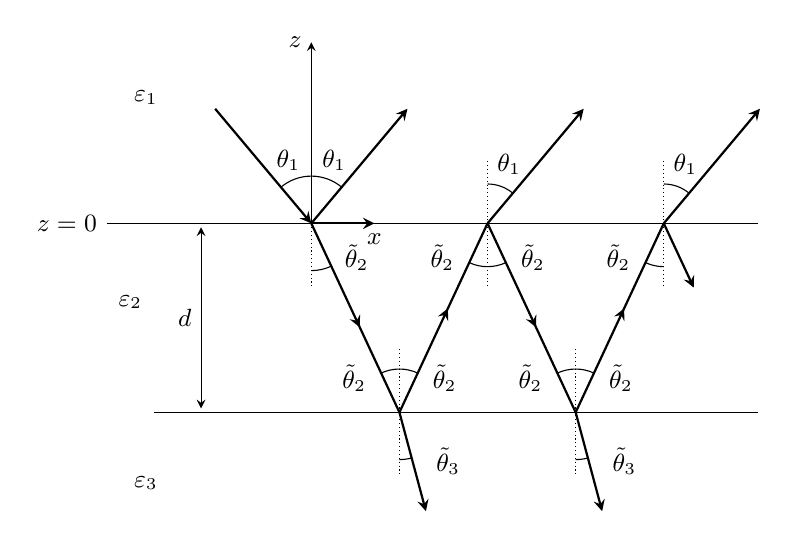
\begin{tikzpicture}[>=stealth, font=\small,
		mid/.style={postaction={decorate}, decoration={markings, mark=at position 0.55 with {\arrow{>}}}}]
		\def\ta{40}\def\tb{25}\def\tc{15}\def\D{2.4}\def\L{1.9}
		\pgfmathsetmacro{\dx}{\D*tan(\tb)}
		\coordinate (T1) at (0,0);
		\coordinate (B1) at (\dx,-\D);
		\coordinate (T2) at ({2*\dx},0);
		\coordinate (B2) at ({3*\dx},-\D);
		\coordinate (T3) at ({4*\dx},0);
		% interfaces and labels
		\draw (-2.6,0) -- ({4*\dx+1.2},0);
		\draw ({-2.0},-\D) -- ({4*\dx+1.2},-\D);
		\node[left] at (-2.6,0) {$z = 0$};
		\node at (-2.1,1.6) {$\varepsilon_1$};
		\node at (-2.3,-1.0) {$\varepsilon_2$};
		\node at (-2.1,-3.3) {$\varepsilon_3$};
		\draw[<->] (-1.4,-0.05) -- (-1.4,{-\D+0.05});
		\node[left] at (-1.4,{-\D/2}) {$d$};
		% z axis and x arrow
		\draw[->] (T1) -- (0,2.3) node[left] {$z$};
		\draw[->, thick] (T1) -- (0.8,0) node[below] {$x$};
		% dotted normals
		\foreach \P in {T2,T3} \draw[densely dotted] ($(\P)+(0,-0.8)$) -- ($(\P)+(0,0.8)$);
		\draw[densely dotted] (T1) -- (0,-0.8);
		\foreach \P in {B1,B2} \draw[densely dotted] ($(\P)+(0,0.8)$) -- ($(\P)+(0,-0.8)$);
		% incident and reflected
		\draw[->, thick] ({-\L*sin(\ta)},{\L*cos(\ta)}) -- (T1);
		\draw[->, thick] (T1) -- ++({90-\ta}:\L);
		% zigzag in the layer
		\draw[thick, mid] (T1) -- (B1);
		\draw[thick, mid] (B1) -- (T2);
		\draw[thick, mid] (T2) -- (B2);
		\draw[thick, mid] (B2) -- (T3);
		% transmitted into medium 1 and 3, and the downward reflection at T3
		\draw[->, thick] (T2) -- ++({90-\ta}:\L);
		\draw[->, thick] (T3) -- ++({90-\ta}:\L);
		\draw[->, thick] (T3) -- ++({270+\tb}:0.9);
		\draw[->, thick] (B1) -- ++({270+\tc}:1.3);
		\draw[->, thick] (B2) -- ++({270+\tc}:1.3);
		% angle arcs: T1
		\draw ([shift={(90:0.6)}]T1) arc (90:{90+\ta}:0.6);
		\draw ([shift={(90:0.6)}]T1) arc (90:{90-\ta}:0.6);
		\node at ($(T1)+({90+\ta/2}:0.85)$) {$\theta_1$};
		\node at ($(T1)+({90-\ta/2}:0.85)$) {$\theta_1$};
		\draw ([shift={(270:0.6)}]T1) arc (270:{270+\tb}:0.6);
		\node at ($(T1)+({270+\tb+28}:0.72)$) {$\tilde{\theta}_2$};
		% B1 and B2
		\foreach \P in {B1,B2} {
			\draw ([shift={(90:0.55)}]\P) arc (90:{90+\tb}:0.55);
			\draw ([shift={(90:0.55)}]\P) arc (90:{90-\tb}:0.55);
			\node at ($(\P)+({90+\tb+28}:0.72)$) {$\tilde{\theta}_2$};
			\node at ($(\P)+({90-\tb-28}:0.72)$) {$\tilde{\theta}_2$};
			\draw ([shift={(270:0.6)}]\P) arc (270:{270+\tc}:0.6);
			\node at ($(\P)+(0.62,-0.62)$) {$\tilde{\theta}_3$};
		}
		% T2
		\draw ([shift={(90:0.5)}]T2) arc (90:{90-\ta}:0.5);
		\node at ($(T2)+({90-\ta/2}:0.8)$) {$\theta_1$};
		\draw ([shift={(270:0.55)}]T2) arc (270:{270-\tb}:0.55);
		\draw ([shift={(270:0.55)}]T2) arc (270:{270+\tb}:0.55);
		\node at ($(T2)+({270-\tb-28}:0.72)$) {$\tilde{\theta}_2$};
		\node at ($(T2)+({270+\tb+28}:0.72)$) {$\tilde{\theta}_2$};
		% T3
		\draw ([shift={(90:0.5)}]T3) arc (90:{90-\ta}:0.5);
		\node at ($(T3)+({90-\ta/2}:0.8)$) {$\theta_1$};
		\draw ([shift={(270:0.55)}]T3) arc (270:{270-\tb}:0.55);
		\node at ($(T3)+({270-\tb-28}:0.72)$) {$\tilde{\theta}_2$};
	\end{tikzpicture}
	\caption{A layer (medium 2, $\varepsilon_2$) of thickness $d$ between medium 1 ($\varepsilon_1$) and a half space (medium 3, $\varepsilon_3$). The incident ray is partly reflected at $z = 0$ and partly transmitted into the layer, where it is reflected back and forth between the two interfaces, transmitting into media 1 and 3 at each encounter.}
	\label{f:layer}
\end{figure}
% NOTE: the second caption sentence is an added description of the sketch.

\begin{itemize}
	% NOTE: handwritten reads "define an effective reflectivity ... in terms of total upward propagating E fields";
	% added "(through the effective reflection coefficient rho; Gamma = |rho|^2)" because the E-field ratio is the
	% reflection coefficient and the reflectivity is its squared magnitude (Lecture 4; U&L 2014, p. 67).
	% The effective reflection coefficient rho = B_1/A_1 (Eq. e:rho_def) is defined, and Eq. (e:rho) is exact, for any d
	% (U&L 2014, Eqs. 2.137-2.138); the conditions below are those for which the lower interface contributes
	% appreciably (cf. Implications 2 and 3 in Section s:implications). Kept as written.
	\item If $d$ is sufficiently small (defined later, but intuition \ldots), and
	\begin{itemize}
		\item the reflectivity at interface 12 is sufficiently small and
		\item the reflectivity at interface 23 is sufficiently large,
	\end{itemize}
	then we can
	\begin{itemize}
		\item[$\rightarrow$] define an effective reflectivity of the two-layer composite in terms of the total upward-\hspace{0pt}propagating $\mathbf{E}$ fields in medium 1 (through the effective reflection coefficient $\rho_\mathrm{eff}$; $\Gamma = |\rho_\mathrm{eff}|^2$).
	\end{itemize}
	% NOTE: handwritten "we can" is inserted with a caret before "define".
	\item Generally, we can define the reflectivity of an $N$-layer composite by defining the dielectric properties and applying the BCs at the $N-1$ interfaces.
	\begin{itemize}
		\item[$\rightarrow$] This can be constructed in a convenient matrix form for straightforward calculation of the effective reflectivity of the $N$-layer structure and the transmission into the bottom layer (the propagation matrix method; Ulaby \& Long 2014, Sec.~2-10.2).
		% NOTE: added "(the propagation matrix method; Ulaby & Long 2014, Sec. 2-10.2)".
		\item[$\rightarrow$] Here, we consider only the 3 layers pictured above (Figure~\ref{f:layer}).
	\end{itemize}
\end{itemize}

\subsection{Fields in medium 1}

% NOTE: handwritten writes the fields without tildes and uses capital K_0; written as phasors (D12) with k_0 (D14).
% Checked against U&L 2014, Eqs. 2.121-2.125 (pp. 64-65), which use -jk_1 for the lossless medium 1 in place of
% -gamma_1 here, and against Lecture 5, Eqs. (e:h_i) and (e:h_r).
\begin{itemize}
	\item Consider an H-polarized incident $\mathbf{E}$ field
	\begin{equation}
		\label{e:E1m}
		\tilde{\mathbf{E}}_1^- = \hat{\mathbf{y}}A_1\,e^{-\gamma_1(x\sin\theta_1 - z\cos\theta_1)},
	\end{equation}
	% NOTE: handwritten reads "we were calling this E_{0h}^i last class"; the typeset Lecture 5 writes E_h^i (D27).
	where
	\begin{itemize}
		\item $A_1$ is the amplitude of the incident field (we called this $E_h^i$ last lecture; simplified here);
		\item note that the superscript $-$ sign indicates downward propagation;
		\item note the use of numerical subscripts instead of $i$, $t$, $r$ $\rightarrow$ to avoid confusion;
		% NOTE: consistent with Lecture 2 (gamma = j omega sqrt(mu_0 eps eps_0) = j k_0 sqrt(eps)).
		\item note that $\gamma_1 \equiv jk_0\sqrt{\varepsilon_1}$.
	\end{itemize}
	\item The upward-propagating wave in medium 1 is
	\begin{equation}
		\label{e:E1p}
		\tilde{\mathbf{E}}_1^+ = \hat{\mathbf{y}}B_1\,e^{-\gamma_1(x\sin\theta_1 + z\cos\theta_1)} = \hat{\mathbf{y}}\rho_\mathrm{eff} A_1\,e^{-\gamma_1(x\sin\theta_1 + z\cos\theta_1)},
	\end{equation}
	where
	\begin{itemize}
		\item $B_1 \equiv$ amplitude of the sum of all upward $\mathbf{E}$ fields;
		\item note that the superscript $+$ indicates upward propagation;
		\item[] \fbox{$\displaystyle \rho_\mathrm{eff} = \frac{B_1}{A_1} \equiv \text{effective reflection coefficient}$} \refstepcounter{equation}\label{e:rho_def}\hfill(\theequation)
	\end{itemize}
	\item The total $\mathbf{E}$ field in medium 1 is
	\begin{equation}
		\tilde{\mathbf{E}}_1 = \tilde{\mathbf{E}}_1^- + \tilde{\mathbf{E}}_1^+ = \hat{\mathbf{y}}A_1\left(e^{\gamma_1z\cos\theta_1} + \rho_\mathrm{eff}\,e^{-\gamma_1z\cos\theta_1}\right)e^{-\gamma_1x\sin\theta_1}.
	\end{equation}
	% NOTE: added "applied to each of the downward- and upward-propagating waves" (the two waves have different
	% propagation unit vectors) and "(Lecture 2)".
	\item We know that $\tilde{\mathbf{H}} = \frac{1}{\eta}\left(\hat{\mathbf{k}}\times\tilde{\mathbf{E}}\right)$ (Lecture 2), applied to each of the downward- and upward-propagating waves
	\item[] $\Rightarrow$ the total magnetic field in medium 1 is
	\begin{align}
		\tilde{\mathbf{H}}_1 &= \hat{\mathbf{x}}\tilde{H}_{1x} + \hat{\mathbf{z}}\tilde{H}_{1z}, \\
		\tilde{H}_{1x} &= \frac{A_1\cos\theta_1}{\eta_1}\left(e^{\gamma_1z\cos\theta_1} - \rho_\mathrm{eff}\,e^{-\gamma_1z\cos\theta_1}\right)e^{-\gamma_1x\sin\theta_1}, \label{e:H1x}\\
		\tilde{H}_{1z} &= \frac{A_1\sin\theta_1}{\eta_1}\left(e^{\gamma_1z\cos\theta_1} + \rho_\mathrm{eff}\,e^{-\gamma_1z\cos\theta_1}\right)e^{-\gamma_1x\sin\theta_1}.
	\end{align}
\end{itemize}

\subsection{Fields in media 2 and 3}

% NOTE: checked against U&L 2014, Eqs. 2.126-2.131 (p. 65). U&L write eta_{c2}, eta_{c3} for the (possibly complex)
% impedances. The handwritten H_{2z} is cut off at the bottom of page L3; completed from U&L Eq. 2.128b (it follows
% from H_{1z} with 1 -> 2 and rho A_1 -> B_2).
% NOTE: added the sentence on complex angles. In lossy media, theta_2 and theta_3 are complex valued (they follow from
% gamma_1 sin theta_1 = gamma_2 sin theta_2 = gamma_3 sin theta_3, Eq. e:snell3); Lecture 5 marks the complex angle
% of refraction with a tilde, but the handwriting and U&L (Eqs. 2.119-2.120) write theta_2, theta_3; kept as written
% (master table D41, pending).
\begin{itemize}
	\item In medium 2, we can follow the same procedure to get
	\begin{align}
		\tilde{\mathbf{E}}_2 &= \tilde{\mathbf{E}}_2^- + \tilde{\mathbf{E}}_2^+ = \hat{\mathbf{y}}\left(A_2\,e^{\gamma_2z\cos\tilde{\theta}_2} + B_2\,e^{-\gamma_2z\cos\tilde{\theta}_2}\right)e^{-\gamma_2x\sin\tilde{\theta}_2}, \\
		\tilde{\mathbf{H}}_2 &= \hat{\mathbf{x}}\tilde{H}_{2x} + \hat{\mathbf{z}}\tilde{H}_{2z}, \\
		\tilde{H}_{2x} &= \frac{\cos\tilde{\theta}_2}{\eta_2}\left(A_2\,e^{\gamma_2z\cos\tilde{\theta}_2} - B_2\,e^{-\gamma_2z\cos\tilde{\theta}_2}\right)e^{-\gamma_2x\sin\tilde{\theta}_2}, \\
		\tilde{H}_{2z} &= \frac{\sin\tilde{\theta}_2}{\eta_2}\left(A_2\,e^{\gamma_2z\cos\tilde{\theta}_2} + B_2\,e^{-\gamma_2z\cos\tilde{\theta}_2}\right)e^{-\gamma_2x\sin\tilde{\theta}_2}.
	\end{align}
	\item In medium 3, there is only downward propagation:
	\begin{align}
		\tilde{\mathbf{E}}_3 &= \hat{\mathbf{y}}\left(A_3\,e^{\gamma_3z\cos\tilde{\theta}_3}\right)e^{-\gamma_3x\sin\tilde{\theta}_3}, \\
		\tilde{\mathbf{H}}_3 &= \hat{\mathbf{x}}\tilde{H}_{3x} + \hat{\mathbf{z}}\tilde{H}_{3z}, \\
		\tilde{H}_{3x} &= \frac{\cos\tilde{\theta}_3}{\eta_3}A_3\,e^{\gamma_3z\cos\tilde{\theta}_3}\,e^{-\gamma_3x\sin\tilde{\theta}_3}, \\
		\tilde{H}_{3z} &= \frac{\sin\tilde{\theta}_3}{\eta_3}A_3\,e^{\gamma_3z\cos\tilde{\theta}_3}\,e^{-\gamma_3x\sin\tilde{\theta}_3}.
	\end{align}
	\item In lossy media, $\tilde{\theta}_2$ and $\tilde{\theta}_3$ are complex valued (cf.\ $\tilde{\theta}_t$ in Lecture 5).
\end{itemize}

\subsection{Applying the BCs}

% NOTE: checked against U&L 2014, Eqs. 2.119a, 2.132-2.136 (pp. 64-66).
\begin{itemize}
	\item Tangential $\mathbf{E}$ field continuous:
	\begin{equation}
		\tilde{\mathbf{E}}_1\big|_{z=0} = \tilde{\mathbf{E}}_2\big|_{z=0}
		\quad\Rightarrow\quad
		\left(A_1 + B_1\right)e^{-\gamma_1x\sin\theta_1} = \left(A_2 + B_2\right)e^{-\gamma_2x\sin\tilde{\theta}_2}.
	\end{equation}
	\item Snell's law:
	\begin{equation}
		\label{e:snell3}
		\gamma_1\sin\theta_1 = \gamma_2\sin\tilde{\theta}_2 = \gamma_3\sin\tilde{\theta}_3
	\end{equation}
	\begin{equation}
		\label{e:bc1}
		\Rightarrow\quad \boxed{A_1 + B_1 = A_2 + B_2}
	\end{equation}
	\item Tangential $\mathbf{H}$ field continuous:
	\begin{equation}
		\tilde{H}_{1x}\big|_{z=0} = \tilde{H}_{2x}\big|_{z=0}
		\quad\Rightarrow\quad
		\boxed{\frac{\cos\theta_1}{\eta_1}\left(A_1 - B_1\right) = \frac{\cos\tilde{\theta}_2}{\eta_2}\left(A_2 - B_2\right)}
		\label{e:bc2}
	\end{equation}
	\item Similarly, at the 23 boundary,
	\begin{equation}
		\tilde{\mathbf{E}}_2\big|_{z=-d} = \tilde{\mathbf{E}}_3\big|_{z=-d}
		\qquad\text{and}\qquad
		\tilde{H}_{2x}\big|_{z=-d} = \tilde{H}_{3x}\big|_{z=-d}
	\end{equation}
	\begin{equation}
		\label{e:bc34}
		\Rightarrow\quad
		\boxed{\begin{aligned}
			&A_2\,e^{-\gamma_2d\cos\tilde{\theta}_2} + B_2\,e^{\gamma_2d\cos\tilde{\theta}_2} = A_3\,e^{-\gamma_3d\cos\tilde{\theta}_3}\\
			&\frac{\cos\tilde{\theta}_2}{\eta_2}\left(A_2\,e^{-\gamma_2d\cos\tilde{\theta}_2} - B_2\,e^{\gamma_2d\cos\tilde{\theta}_2}\right) = \frac{A_3\cos\tilde{\theta}_3}{\eta_3}\,e^{-\gamma_3d\cos\tilde{\theta}_3}
		\end{aligned}}
	\end{equation}
\end{itemize}

\subsection{Effective reflection coefficient of the two-layer composite}

\begin{itemize}
	\item Assuming $A_1$ is known, Eqs.~\eqref{e:bc1}--\eqref{e:bc34} are 4 equations in 4 unknowns ($B_1$, $A_2$, $B_2$, $A_3$).
	% NOTE: checked against U&L 2014, Eqs. 2.138-2.140 (p. 66), and numerically (python3): a direct solve of the four
	% BC equations (H pol.) and of the corresponding TM equations (V pol., with the Lecture 5 reference directions,
	% Fig. f:pol) agrees with Eq. (e:rho) to machine precision for lossless and lossy layers, e.g., eps = 1,
	% 3.2 - j0.2, 87 - j58 at 30 deg and 70 deg (U&L's ice-over-sea example), and eps_1 = 2 > eps_3 = 1.5.
	% Limits (python3): d -> 0 gives rho_13; eps_2 = eps_3 gives rho_12; a lossy layer with d >> delta_s gives rho_12;
	% eps_2 = eps_1 gives rho_13 exp(-2 gamma_1 d cos theta_1), i.e., the single interface shifted to z = -d
	% (|rho| = |rho_13| for lossless medium 1); lossless half-wave layer (2 beta_2 d cos theta_2 = 2 pi) gives rho_13, and
	% quarter-wave gives (rho_12 - rho_23)/(1 - rho_12 rho_23). For lossless stacks, |rho|^2 + T = 1 for both
	% polarizations (T from A_3; python3).
	\item Grinding through the algebra gives
	\begin{equation}
		\label{e:rho}
		\boxed{\rho_\mathrm{eff} = \frac{\rho_{12} + \rho_{23}\,e^{-2\gamma_2d\cos\tilde{\theta}_2}}{1 + \rho_{12}\rho_{23}\,e^{-2\gamma_2d\cos\tilde{\theta}_2}}}
	\end{equation}
	where the Fresnel reflection coefficients (Lecture 5) at the two interfaces are
	\begin{equation}
		\label{e:rho12}
		\rho_{12} =
		\begin{cases}
			\dfrac{\eta_2\cos\theta_1 - \eta_1\cos\tilde{\theta}_2}{\eta_2\cos\theta_1 + \eta_1\cos\tilde{\theta}_2} & \text{H pol.},\\[12pt]
			\dfrac{\eta_2\cos\tilde{\theta}_2 - \eta_1\cos\theta_1}{\eta_2\cos\tilde{\theta}_2 + \eta_1\cos\theta_1} & \text{V pol.},
		\end{cases}
	\end{equation}
	\begin{equation}
		\label{e:rho23}
		\rho_{23} =
		\begin{cases}
			\dfrac{\eta_3\cos\tilde{\theta}_2 - \eta_2\cos\tilde{\theta}_3}{\eta_3\cos\tilde{\theta}_2 + \eta_2\cos\tilde{\theta}_3} & \text{H pol.},\\[12pt]
			\dfrac{\eta_3\cos\tilde{\theta}_3 - \eta_2\cos\tilde{\theta}_2}{\eta_3\cos\tilde{\theta}_3 + \eta_2\cos\tilde{\theta}_2} & \text{V pol.}
		\end{cases}
	\end{equation}
	% NOTE: added "(Lecture 5)" and "(as in Eqs. e:rho_h and e:rho_v of Lecture 5, with 1 -> ..."; handwritten brace label
	% reads "Fresnel ref. coefs".
	These have the forms of $\rho_h$ and $\rho_v$ in Lecture 5, with media $1\rightarrow2$ ($\rho_{12}$) and $2\rightarrow3$ ($\rho_{23}$).
\end{itemize}

%%%%%%%%%%%%%%%%%%%%%%%%%%%%%%%%%%%%%
\section{A more direct approach: multiple reflections}
\label{s:multiple}

But, now that we've laid the groundwork, let's take a more direct approach (dropping the $x$ component of the phase because Snell's law tells us that the $x$ values are constant in all media); see Figure~\ref{f:multiple}.


\begin{figure}[!hbp]
	\centering
	% Elements follow the handwritten sketch: labels "incident wave", "H polarized", medium 1/2/3, z = 0, z = -d; the
	% incident ray (amplitude 1), reflected rho_12, zigzag in the layer with direction arrows and the amplitude labels
	% placed as in the sketch (near the start and end of each segment), rays transmitted into medium 1 with their
	% amplitudes, the downward reflection at the third top point, unlabeled rays transmitted into medium 3, and the
	% definition of Phi. The amplitude arriving back at the third top point is unlabeled in the sketch.
	% Illustrative angles: theta_1 = 45 deg, theta_2 ~ 33 deg (dx/D = 2.2/3.4).
	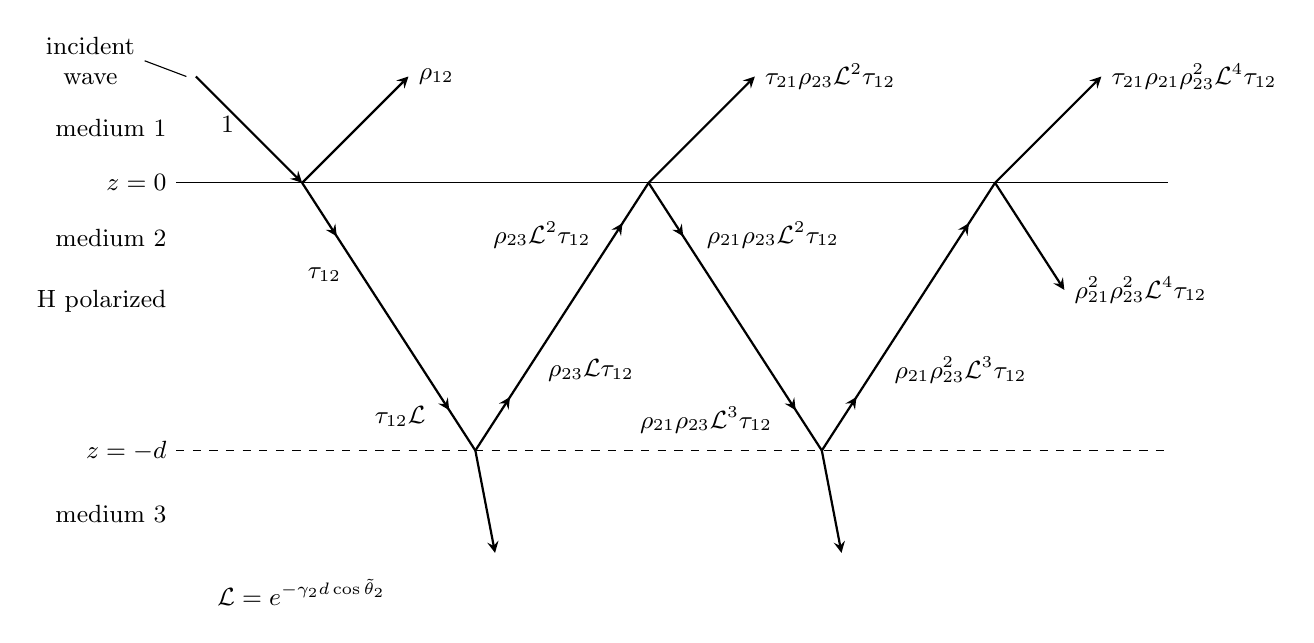
\begin{tikzpicture}[>=stealth, font=\small,
		mid/.style={postaction={decorate}, decoration={markings, mark=at position 0.2 with {\arrow{>}}, mark=at position 0.85 with {\arrow{>}}}}]
		\def\D{3.4}\def\dx{2.2}\def\L{1.35}
		\coordinate (T1) at (0,0);
		\coordinate (B1) at (\dx,-\D);
		\coordinate (T2) at ({2*\dx},0);
		\coordinate (B2) at ({3*\dx},-\D);
		\coordinate (T3) at ({4*\dx},0);
		\draw (-1.6,0) -- ({4*\dx+2.2},0);
		\draw[dashed] (-1.6,-\D) -- ({4*\dx+2.2},-\D);
		\node[left] at (-1.6,0) {$z = 0$};
		\node[left] at (-1.6,-\D) {$z = -d$};
		\node[left] at (-1.6,0.7) {medium 1};
		\node[left] at (-1.6,-0.7) {medium 2};
		\node[left] at (-1.6,-1.5) {H polarized};
		\node[left] at (-1.6,-4.2) {medium 3};
		% incident and reflected
		\draw[->, thick] (-\L,\L) -- (T1);
		\node[left, align=center] (iw) at (-2.0,{\L+0.2}) {incident\\wave};
		\draw (iw.east) -- ({-\L-0.12},\L);
		\node[left] at ({-0.55*\L},{0.55*\L}) {1};
		\draw[->, thick] (T1) -- ++(\L,\L) node[right] {$\rho_{12}$};
		% zigzag
		\draw[thick, mid] (T1) -- (B1);
		\draw[thick, mid] (B1) -- (T2);
		\draw[thick, mid] (T2) -- (B2);
		\draw[thick, mid] (B2) -- (T3);
		% transmitted up, reflected down at T3, transmitted into medium 3
		\draw[->, thick] (T2) -- ++(\L,\L) node[right] {$\tau_{21}\rho_{23}\mathcal{L}^2\tau_{12}$};
		\draw[->, thick] (T3) -- ++(\L,\L) node[right] {$\tau_{21}\rho_{21}\rho_{23}^2\mathcal{L}^4\tau_{12}$};
		\draw[->, thick] (T3) -- ++({0.4*\dx},{-0.4*\D}) node[right] {$\rho_{21}^2\rho_{23}^2\mathcal{L}^4\tau_{12}$};
		\draw[->, thick] (B1) -- ++(0.25,-1.3);
		\draw[->, thick] (B2) -- ++(0.25,-1.3);
		% segment labels
		\node[anchor=north east] at ($(T1)!0.28!(B1)$) {$\tau_{12}$};
		\node[anchor=north east, xshift=-2pt] at ($(T1)!0.8!(B1)$) {$\tau_{12}\mathcal{L}$};
		\node[anchor=west, xshift=4pt] at ($(B1)!0.3!(T2)$) {$\rho_{23}\mathcal{L}\tau_{12}$};
		\node[anchor=south east] at ($(B1)!0.72!(T2)$) {$\rho_{23}\mathcal{L}^2\tau_{12}$};
		\node[anchor=south west] at ($(T2)!0.28!(B2)$) {$\rho_{21}\rho_{23}\mathcal{L}^2\tau_{12}$};
		\node[anchor=north east, xshift=-2pt] at ($(T2)!0.8!(B2)$) {$\rho_{21}\rho_{23}\mathcal{L}^3\tau_{12}$};
		\node[anchor=west, xshift=4pt] at ($(B2)!0.3!(T3)$) {$\rho_{21}\rho_{23}^2\mathcal{L}^3\tau_{12}$};
		% Phi
		\node[anchor=west] at (-1.2,-5.2) {$\mathcal{L} = e^{-\gamma_2d\cos\tilde{\theta}_2}$};
	\end{tikzpicture}
	\caption{Multiple reflections of an H-polarized wave of unit amplitude incident from medium 1 on the layer (medium 2). Each label gives the amplitude of the wave at that point (the $x$ component of the phase is dropped). $\rho_{12}$ and $\tau_{12}$ are the reflection and transmission coefficients for incidence from medium 1 on medium 2 (similarly $\rho_{21}$, $\rho_{23}$, $\tau_{21}$), and $\mathcal{L}$ is the propagation factor across the layer.}
	\label{f:multiple}
\end{figure}
% NOTE: the caption's second and third sentences are added descriptions. The labels match U&L 2014, Fig. 2-24 (p. 68,
% with L for Phi), except U&L's label (checked on a 300-dpi render) on the second transmitted ray, tau_21 rho_21^2 L^4 tau_12, which should read
% tau_21 rho_21 rho_23^2 L^4 tau_12 (as handwritten here and in U&L Eq. 2.141).

\subsection{Summing the multiple reflections}

% NOTE: checked against U&L 2014, Sec. 2-10.3, Eqs. 2.141-2.143 (p. 67), and numerically (python3: partial sums of the
% series converge to Eq. e:rho, H and V pol.). U&L write L (script) for the propagation factor and x for chi.
\begin{itemize}
	\item Now, summing all upward-going waves in medium 1,
	\begin{align}
		\rho_\mathrm{eff} &= \rho_{12} + \tau_{21}\rho_{23}\mathcal{L}^2\tau_{12} + \tau_{21}\rho_{21}\rho_{23}^2\mathcal{L}^4\tau_{12} + \cdots \nonumber\\
		&= \rho_{12} + \tau_{12}\tau_{21}\rho_{23}\mathcal{L}^2\sum_{p=0}^{\infty}\chi^p,
	\end{align}
	% NOTE: handwritten symbol reads as a cursive x (possibly chi; low confidence); U&L Eq. 2.141 uses x. Written chi
	% because x is reserved for the Cartesian coordinate (master table D13).
	where
	\begin{equation}
		\chi = \rho_{21}\rho_{23}\mathcal{L}^2.
	\end{equation}
	% NOTE: handwritten reads "|Phi^2| < 1"; corrected to |Phi^2| <= 1 because |Phi^2| = exp[-2 Re(gamma_2 cos theta_2) d]
	% = 1 for a lossless layer (gamma_2 = j beta_2, real theta_2). U&L 2014, p. 67, make the same "smaller than 1" claim
	% for L^2, which likewise fails for a lossless layer. |chi| < 1 still follows from |rho_21| < 1.
	% Added the scope "(medium 1 air, ...)": a random search (python3; 3x10^5 cases with eps_1 = 1, eps_2' and
	% eps_3' in 1-90, eps'' in 0-60, theta_1 < 90 deg, both polarizations) found max |rho_21| = 0.99996,
	% max |rho_23| = 0.973, max |chi| = 0.97. Outside this scope the bounds can fail: e.g., eps_1 = 2.83,
	% eps_2 = 1.43, eps_3 = 2.38 - j6.91, V pol., theta_1 = 47.8 deg (total internal reflection at interface 12)
	% gives |chi| = 1.64 at d = 0, 1.41 at d = 1 cm, and 0.78 at d = 5 cm (f = 1 GHz), so the series can diverge, but Eq. (e:rho) still holds (direct BC solve, python3).
	\item Note that $|\rho_{21}| < 1$, $|\rho_{23}| < 1$, and $|\mathcal{L}^2| \le 1$ (with equality for a lossless layer)
	\item[] $\Rightarrow$ $|\chi| < 1$ (for medium 1 air, media with $\varepsilon' \ge 1$, and $\theta_1 < 90^\circ$).
	\item Also,
	\begin{equation}
		\rho_{21} = -\rho_{12} \quad\rightarrow\quad \tau_{21} = 1 + \rho_{21} = 1 - \rho_{12}.
	\end{equation}
	Recall that
	\begin{equation}
		\tau_{12} = 1 + \rho_{12}.
	\end{equation}
	% NOTE: these tau relations are for H polarization (Lecture 5, Eq. e:tau_h), as in the sketch. For V polarization,
	% tau_12 = (1 + rho_12) cos theta_1/cos theta_2 and tau_21 = (1 + rho_21) cos theta_2/cos theta_1 (Lecture 5,
	% Eq. e:tau_v; U&L p. 67), so the product tau_12 tau_21 = (1 + rho_12)(1 - rho_12) is the same and the result below
	% holds for both polarizations (verified numerically, python3).
	\item Use the identity (Taylor series)
	\begin{equation}
		\sum_{p=0}^{\infty}\chi^p = \frac{1}{1-\chi}
	\end{equation}
	\begin{equation}
		\Rightarrow\quad \rho_\mathrm{eff} = \rho_{12} + \frac{\left(1+\rho_{12}\right)\left(1-\rho_{12}\right)\rho_{23}\mathcal{L}^2}{1 + \rho_{12}\rho_{23}\mathcal{L}^2}
	\end{equation}
	\begin{equation}
		\Rightarrow\quad \boxed{\rho_\mathrm{eff} = \frac{\rho_{12} + \rho_{23}\,e^{-2\gamma_2d\cos\tilde{\theta}_2}}{1 + \rho_{12}\rho_{23}\,e^{-2\gamma_2d\cos\tilde{\theta}_2}}}
	\end{equation}
	the same result as Eq.~\eqref{e:rho}.
	% NOTE: added "the same result as Eq. (e:rho)".
\end{itemize}

\subsection{Implications}
\label{s:implications}

\begin{enumerate}
	% NOTE: added "(the wavelength in medium 2)". The oscillation comes from the phase factor exp(-j 2 beta_2 d cos theta_2);
	% |rho| oscillates in d with period lambda_2/(2 cos theta_2) (low-loss layer; python3: 8.38 cm for eps_2 = 3.2 - j0.2
	% at 1 GHz, normal incidence, matching lambda_2/2 and U&L 2014, Fig. 2-22a, p. 66; 8.98 cm = lambda_2/(2 cos theta_2)
	% for eps_2 = 3.2 at theta_1 = 40 deg, both polarizations).
	\item $\gamma_2$ is complex valued, so for $d \gtrsim \lambda_2$ (the wavelength in medium 2), $|\rho_\mathrm{eff}|$ should have oscillatory behavior, with maxima corresponding to constructive interference of the multiple reflections and minima $\rightarrow$ destructive interference.
	% NOTE: |Phi^2| = exp[-2 Re(gamma_2 cos theta_2) d] and Re(gamma_2 cos theta_2) >= alpha_2 = 1/delta_s for medium 1
	% air (python3, 2x10^5 random lossy layers), so the second terms of Eq. (e:rho) vanish for d >> delta_s.
	\item For $d \gg \delta_s$, $\rho_\mathrm{eff} \rightarrow \rho_{12}$.
	\item For $\rho_{23} \ll 1$, $\rho_\mathrm{eff} \rightarrow \rho_{12}$.
\end{enumerate}

%%%%%%%%%%%%%%%%%%%%%%%%%%%%%%%%%%%%%
% Symbols follow the master table in ../variables_master.tex; see it for flagged dual usages.
\section*{Variables}

Units are SI. Values are given for universal constants; ``typical'' values are representative, not definitive.

{\small
\renewcommand{\arraystretch}{1.25}
\begin{longtable}{>{$}l<{$} >{\raggedright\arraybackslash}p{0.37\textwidth} >{\raggedright\arraybackslash}p{0.15\textwidth} >{\raggedright\arraybackslash}p{0.24\textwidth}}
\hline
\textrm{Symbol} & Description & Units & Value \\
\hline
\endfirsthead
\hline
\textrm{Symbol} & Description & Units & Value \\
\hline
\endhead
\hline
\endfoot
\multicolumn{4}{l}{\emph{Constants and wavenumber}} \\
j & imaginary unit, $j^2 = -1$ (time dependence $e^{j\omega t}$) & -- & -- \\
k_0 & free-space angular wavenumber & rad/m & -- \\
\multicolumn{4}{l}{\emph{Constitutive parameters}} \\
\varepsilon_1,\ \varepsilon_2,\ \varepsilon_3 & complex dielectric constants (relative) of media 1, 2, 3, $\varepsilon' - j\varepsilon''$; real parts $\varepsilon_1'$, $\varepsilon_2'$, $\varepsilon_3'$ & dimensionless & -- \\
\varepsilon_1',\ \varepsilon_2' & relative permittivities of media 1 and 2 & dimensionless & $\ge 1$ (almost always) \\
\mu_1,\ \mu_2 & permeabilities of media 1 and 2 & H/m & $\mu_0$ in RS \\
\multicolumn{4}{l}{\emph{Boundary conditions and geometric optics}} \\
\mathbf{E}_1,\ \mathbf{E}_2 & (total) electric field in media 1 and 2 & V/m & -- \\
\mathbf{H}_1,\ \mathbf{H}_2 & (total) magnetic field in media 1 and 2 & A/m & -- \\
E^\perp,\ H^\perp & field components normal to the interface & V/m; A/m & -- \\
\mathbf{E}^\parallel,\ \mathbf{H}^\parallel & field components tangential to the interface & V/m; A/m & -- \\
\hat{\mathbf{a}} & unit normal to the interface & dimensionless & -- \\
\theta_i,\ \theta_r & angles of incidence and reflection & rad & $\theta_i = \theta_r = \theta_1$ \\
\multicolumn{4}{l}{\emph{Layered media}} \\
d & thickness of the layer (medium 2) & m & -- \\
N & number of layers in a composite & dimensionless & 3 here \\
x,\ y,\ z & Cartesian coordinates & m & interfaces at $z = 0$, $-d$ \\
\hat{\mathbf{x}},\ \hat{\mathbf{y}},\ \hat{\mathbf{z}} & Cartesian unit vectors & dimensionless & -- \\
\theta_1,\ \tilde{\theta}_2,\ \tilde{\theta}_3 & angles of propagation (from the normal) in media 1, 2, 3 & rad & complex in lossy media (real if lossless) \\
\gamma_1,\ \gamma_2,\ \gamma_3 & propagation constants of media 1, 2, 3, $jk_0\sqrt{\varepsilon}$ & m$^{-1}$ & -- \\
\eta_1,\ \eta_2,\ \eta_3 & intrinsic impedances of media 1, 2, 3 & $\Omega$ & -- \\
\hat{\mathbf{k}} & propagation unit vector & dimensionless & -- \\
\tilde{\mathbf{E}}_1^-,\ \tilde{\mathbf{E}}_1^+ & downward- and upward-propagating $\mathbf{E}$ phasors in medium 1 (likewise medium 2) & V/m & -- \\
\tilde{\mathbf{E}}_1,\ \tilde{\mathbf{E}}_2,\ \tilde{\mathbf{E}}_3 & total $\mathbf{E}$ phasors in media 1, 2, 3 & V/m & -- \\
\tilde{\mathbf{H}}_1,\ \tilde{\mathbf{H}}_2,\ \tilde{\mathbf{H}}_3 & total $\mathbf{H}$ phasors in media 1, 2, 3 & A/m & -- \\
\tilde{H}_{1x},\ \tilde{H}_{1z},\ \ldots & $x$ and $z$ components of $\tilde{\mathbf{H}}_1$ (likewise media 2, 3) & A/m & -- \\
E_h^i & amplitude of the incident H-polarized field (Lecture 5), here $A_1$ & V/m & -- \\
A_1,\ A_2,\ A_3 & amplitudes of the downward-propagating $\mathbf{E}$ fields in media 1, 2, 3 & V/m & $A_1$ known \\
B_1,\ B_2 & amplitudes of the upward-propagating $\mathbf{E}$ fields in media 1 and 2 & V/m & -- \\
\rho_\mathrm{eff} & effective reflection coefficient of the composite, $B_1/A_1$ & dimensionless & $\rho_{12}$ if $d \gg \delta_s$ \\
\Gamma & reflectivity, $|\rho_\mathrm{eff}|^2$ & dimensionless & $0$--$1$ \\
\rho_{12},\ \rho_{23} & Fresnel reflection coefficients for incidence from medium 1 on 2 and from 2 on 3 (H or V pol.) & dimensionless & -- \\
\rho_{21} & Fresnel reflection coefficient for incidence from medium 2 on 1 & dimensionless & $-\rho_{12}$ \\
\tau_{12},\ \tau_{21} & Fresnel transmission coefficients from medium 1 to 2 and from 2 to 1 & dimensionless & H pol.: $1 + \rho_{12}$, $1 - \rho_{12}$ \\
\mathcal{L} & propagation factor across the layer, $e^{-\gamma_2d\cos\tilde{\theta}_2}$ & dimensionless & $|\mathcal{L}| \le 1$ \\
\chi & ratio of successive terms, $\rho_{21}\rho_{23}\mathcal{L}^2$ & dimensionless & $|\chi| < 1$ (medium 1 air, $\varepsilon' \ge 1$, $\theta_1 < 90^\circ$) \\
p & summation index & dimensionless & $0, 1, 2, \ldots$ \\
\lambda_2 & wavelength in medium 2 & m & -- \\
\alpha,\ \alpha_2 & attenuation constant (of medium 2), $\mathrm{Re}(\gamma)$ & Np/m & 0 if lossless \\
\delta_s & skin depth, $1/\alpha$ & m & -- \\
\delta_p & penetration depth, $1/(2\alpha)$ & m & $\delta_s/2$ \\
\end{longtable}
}

\end{document}
